% coding:utf-8
\documentclass[a5paper,10pt,fleqn]{book}

\usepackage[utf8]{inputenc} % für input utf8
\usepackage[T1]{fontenc} %Schriftcodierung mit UTF-8
\usepackage{textcomp} %Erweiterung von fontenc
\usepackage{lmodern} %Erweiterung des Zeichensatzes

\usepackage{graphics}
\usepackage{graphicx}
\usepackage[ngerman]{babel}
\usepackage{amsmath}
%\usepackage[all]{xy}
%\usepackage[xindy]{glossaries}
\usepackage{makeidx}
\usepackage{pdfpages}
\usepackage{graphicx}
\usepackage{hyperref}
\usepackage{amssymb}

\title{Formelsammlung Mathematik}
\author{Daniel Winz, Ervin Malagic}
\date{\today}

\begin{document}

\maketitle

\chapter*{Über diese Arbeit}
Dies ist das Ergebnis einer Zusammenarbeit auf Basis freier Texte erstellt von Studierenden der Fachhochschule Luzern. 

Dieses Schriftstück ist lizenziert unter der GPLv2 und der \TeX-  bzw. \LaTeX- Code ist auf \url{github.com/daniw/fosamath} hinterlegt.


\tableofcontents

\chapter{Vektorgeometrie}
\section{Vektorgeometrie in der Ebene}

\subsection{Anstand zweier Puntke}
\[ \boxed{ \overline{P_1 P_2} = \sqrt{ (x_2 - x_1)^2 + (y_2 - y_1)^2 } } \]

\subsection{Geradengleichungen}

\subsubsection{Normalform (explizite Form)}
\[ \boxed{ g: y= mx + q }\]
\[ \boxed{ \text{Steigung } m = \frac{y_2 - y_1}{x_2 - x_1} = \frac{\Delta y}{\Delta x}  = tan \varphi } \]

\subsubsection{Koordinatenform (implizite Form)}
\[ \boxed{ g: ax + by + c = 0 } \]

\subsubsection{Achsenabschnittsform}
\[ \boxed{ g: \frac{x}{p} + \frac{y}{q} = 1 } \]

\subsubsection{Hesse'sche Normalform}
\[ \boxed{ g:  \frac{ax + by + c}{\sqrt{ a^2 + b^2 } } = 0 }  \]

\subsubsection{Parameterform}
\[ \boxed{ 
    g: \vec{r} = \vec{r_0} + t \cdot \vec{a}  = 
      \left( 
	\begin{array}{cc} 
	  x_0 \\ y_0
	\end{array}
      \right)
      + t \cdot 
      \left( 
	\begin{array}{cc} 
	  a_x \\ a_y
	\end{array}
      \right)  
   }
\]


\subsection{Normalenvektor}
Der Normalenvektor ist ein Vektor, welcher senkrecht auf einem anderen Vektor bzw. einer Geraden liegt. Hier im Beispiel in welchem $ \vec{n} \bot g(x)$
\[ \boxed{ \vec{n} = 
      \left( 
	\begin{array}{cc} 
	  n_x \\ n_y
	\end{array}
      \right)
      =
      \left( 
	\begin{array}{cc} 
	  a \\ b
	\end{array}
      \right)
      =
      \left( 
	\begin{array}{cc} 
	  -a_y \\ a_x
	\end{array}
      \right)
} \]
\noindent
Der Richtungsvektor von $g(x)$ ist 
$  
      \left( 
	\begin{array}{cc} 
	  a_x \\ a_y
	\end{array}
      \right)
      \Rightarrow 
      \left( 
	\begin{array}{cc} 
	  -a_y \\ a_x
	\end{array}
      \right)
      = \vec{n}
$.

\subsection{Abstand Punkt zu Gerade}
Für eine Gerade $g: ax + by + c = 0$ und einen Punkt $P_1 (x_1 | y_1)$ gilt:
\[ \boxed{ d = \left| \frac{ax_1 + by_1 + c}{\sqrt{a^2 + b^2}} \right| } \]

\subsection{Schnittwinkel zwischen Geraden}
Für den spitzen Schnittwinkel $\varphi$ zwischen den Geraden 

$g_1: y = m_1x + q_1$ und $g_2: y = m_2x + q_2$ gilt:
\[ \boxed{ tan\varphi = \left| \frac{m_2 - m_1}{1 + m_1 \cdot m_2} \right| } \\ \text{für } \varphi \neq 90^{\circ} \]

\[ \boxed{ g_1 || g_2 \Leftrightarrow m_1 = m_2 \text{und } g_1 \bot g_2 \Leftrightarrow m_2 = - \frac{1}{m_1} } \\ \text{für } m_1 \neq 0 \]

\section{Vektorgeometrie im Raum}

\subsection{Ortsvektor}
Ein Ortsvektor beschreibt den Vektor vom Urspung des Koordinatensystems $O(0|0|0)$ zu einem beliebigen Punkt $P(x|y|z)$.
\[	\boxed{ \vec{r} = \overrightarrow{OP} = x\vec{e_x} + y\vec{e_y} + z\vec{e_z} :=
	\left( 
	  \begin{array}{ccc} 
	    x \\ y \\ z
	  \end{array}
	\right) }
\]
\noindent
Die Vektoren $\vec{e_x},\vec{e_y},\vec{e_z}$ sind die Einheitsvektoren des Koordinatensystems (meist einfach 1 ohne Einheit).
\subsection{Länge eines Ortsvektors (Betrag)}
\[ \boxed{ |\vec{r}| = r = \sqrt{x^2 + y^2 1 z^2} } \]


\chapter{Folgen und Reihen}
% coding:utf-8

%----------------------------------------
%FOSAMATH, a LaTeX-Code for a mathematical summary for basic analysis
%Copyright (C) 2013, Daniel Winz, Ervin Mazlagic, Adrian Imboden, Philipp Langer

%This program is free software; you can redistribute it and/or
%modify it under the terms of the GNU General Public License
%as published by the Free Software Foundation; either version 2
%of the License, or (at your option) any later version.

%This program is distributed in the hope that it will be useful,
%but WITHOUT ANY WARRANTY; without even the implied warranty of
%MERCHANTABILITY or FITNESS FOR A PARTICULAR PURPOSE.  See the
%GNU General Public License for more details.
%----------------------------------------


% coding:utf-8
\section{Folgen}
$a_1$ (bzw. $a_0$) ist das erste Glied einer Folge\\
$a_n$ ist das $n$-te Glied einer Folge

\subsection{Form}
Eine Folge kann drei spezielle Formen annehmen. Für $(a_n)_{n \in \mathbb{N}}$ 
gilt die Folge je nach dem als
\subsubsection*{monoton wachsend}
$ \boxed{ a_{n+1} \geq a_n \quad \forall \quad n \in \mathbb{N} } $ Bsp.: $a_n 
= 2^n$, $a_{n+1} = 2^{n+1}$
\subsubsection*{monoton fallend}
$ \boxed{ a_{n+1} \leq a_n \quad \forall \quad n \in \mathbb{N} } $ Bsp.: $a_n 
= \frac{1}{n}$, $a_{n+1} = \frac{1}{n+1}$
\subsubsection*{alternierend}
$ \boxed{ a_{n+1} \cdot a_n < 0 } $ Bsp.: $a_n := (-2)^n$, $a_{n+1} 
= (-2)^{n+1} \cdot (-2)^n = (-2)^{2n+1}$\\\\
Bei den monoton wachsend/fallenden Folgen kann noch weiter unterschieden werden 
zwischen streng monoton und einfach monoton. Streng monoton bedeutet dann, dass 
$a_n \neq a_{n+1}$ wobei das bei einfach monotonen der Fall sein kann 
(vgl.~\ref{subsec:monotonie}).
\subsection{rekursive Darstellung}
Bei der rekursiven Darstellung wird eine Folge durch einen Startwert und eine 
Abbildungsvorschrift dargestellt. \\
\[ \boxed{ \begin{matrix}
\text{Startwert} & f(1) = a_1 \\
\text{Vorschrift} & F(f(1), f(2), \ldots, f(n)) := f(n + 1) = a_{n + 1}
\end{matrix}} \]

\subsection{arithmetische Folgen}
$d$ ist die Differenz zwischen zwei benachbarten Gliedern\\
\[ \boxed{d = a_{n+1} - a_n} \]
\[ \boxed{a_{n+1} = a_n + d} \]
\[ \boxed{ \begin{matrix} 
a_0 :& a_n =& a_0 + n \cdot d \\
a_1 :& a_n =& a_1 + (n - 1)d 
\end{matrix}}\]

\subsection{geometrische Folgen}
$q$ ist der Quotient von zwei benachbarten Gliedern\\
\[ \boxed{\frac{a_{n+1}}{a_n} = q} \]
\[ \boxed{a_{n+1} = a_n \cdot q} \]
\[ \boxed{\begin{array}{ll}
a_0 :& a_n = q^{n} a_0\\
a_1 :& a_n = q^{n-1} a_1
\end{array}} \]

\ifti
\subsubsection{Folgen mit dem TI-89}
%seq($a_n$, Variable, $n_1$, $n_2$)\\\\
\verb{seq(EXP,VAR,LOW,HIGH[,STEP]){\\\\
\begin{tabular}{@{}lll}
EXP	& Ausdruck	& bezeichnet den Term \\
VAR 	& Variable	& bezeichnet die inkrementierte Variabel \\
LOW	& untere Grenze	& Anfangspunkt der Inkrementierung \\
HIGH	& obere Grenze	& Endpunkt der Inkrementierung \\
STEP	& n-Schritte	& Zeigt Resultate mit n-ten Schritt
\end{tabular}\\\\
Bsp.: \verb{seq(1/x,x,1,10,5){ erzeugt die Ausgabe \verb?{1   1/6}?
\fi
\ifnspire
\subsubsection{Folgen mit dem TI-Nspire}
seq($a_n$, Variable, $n_1$, $n_2$)\\\\
\begin{tabular}{@{}ll}
$a_n$    & Formel für die Berechnung des n-ten Gliedes\\
Variable & Variable in der Formel\\
$n_1$    & erstes zu berechnendes Glied\\
$n_2$    & letztes zu berechnendes Glied
\end{tabular}
\fi

\subsection{Konvergenz von Folgen}
Eine Folge ist konvergent, wenn der Grenzwert der Folge eine reelle Zahl ist
\[ \boxed{\lim\limits_{n \to \infty} a_n = a \quad a \in \mathbb{R}}\]

\subsubsection{Rechenregeln}
$ a_n \xrightarrow[\rightarrow \infty]{} a $, 
$ b_n \xrightarrow[n \rightarrow \infty]{} b $
\[ \boxed{ a_n + b_n \xrightarrow[]{n \rightarrow \infty} a + b } \]
\[ \boxed{ a_n - b_n \xrightarrow[]{n \rightarrow \infty} a - b } \]
\[ \boxed{ a_n \cdot b_n \xrightarrow[]{n \rightarrow \infty} a \cdot b } \]
\[ \boxed{ \alpha \cdot a_n \xrightarrow[]{n \rightarrow \infty} \alpha \cdot a, 
\quad \alpha \in \mathbb{R} } \]
\[ \boxed{ \frac{a_n}{b_n} \xrightarrow[]{n \rightarrow \infty} \frac{a}{b}, 
\quad \text{falls} \quad b_n \neq 0 \quad \forall \quad n \in \mathbb{N} } \]

\ifti
\subsubsection{Konvergenz von Folgen mit dem TI-89}
Für die Berechnung von Grenzwerten mit dem TI-89 siehe \ref{subsubsec:limti}. 
\fi
\ifnspire
\subsubsection{Konvergenz von Folgen mit dem TI-Nspire}
Für die Berechnung von Grenzwerten mit dem TI-Nspire siehe 
\ref{subsubsec:limnspire}. 
\fi

% coding:utf-8
\section{Reihen}
$S_n$ ist die Summe aller Glieder von $a_1$ bis $a_n$. 
\[ \boxed{S_n = \sum_{k=1}^{n} a_k = a_1 + a_2 + a_3 \cdots + a_n} \]

\subsection{arithmetische Reihe}
\[ \boxed{S_n = \left(n + 1\right)\left(a_0 + d \frac{n}{2}\right) = \left(n + 1\right) \frac{a_0 + a_n}{2}} \]

\subsection{geometrische Reihe}
\[ \boxed{\text{Für } q \neq 1: \quad S_n = a_1 \left(  \frac{q^n - 1}{q - 1} \right) = a_1 \left(  \frac{1 - q^n}{1 - q} \right)} \]

\[ \boxed{\begin{array}{ll}
a_0 :& S_n = a_0 \cdot \dfrac{1-q^{n+1}}{1-q} \\ 
& \\
a_1 :& S_n = a_1 \cdot \dfrac{1-q^n}{1-q}
\end{array}} \]

\[ \boxed{\text{Für } q = 1: \quad S_n = a_1 \left(1+1^1 + 1^2 + \ldots + 1^{n-1}\right) = a_1 n} \]
Unendliche geometrische Reihe
\[ \boxed{\text{Für } |q| < 1: S = \lim_{n \rightarrow \infty} S_n = \frac{a_1}{1 - q}} \] 
%Um das $n$-te Glied einer geometrischen Reihen zu berechnen gilt:\\
%$ q = \frac{a_n}{a_{n-1}} = \frac{a_{n-1}}{a_{n-2}} $ \\
%$ \Rightarrow  a_n = a_{(n-1)} \cdot q = a_{(n-2)} \cdot q^2 = a_{(n - (n-1))} \cdot q^{(n-1)} = a_1 \cdot q^{(n-1)} $
%\[ \boxed{ a_n = a_1 \cdot q^{n-1} } \]
%\[ \boxed{ a_{n+1} = a_1 \cdot q^n } \]
$a_1$ ist hier das erste Element der geometrischen Folge!

\subsection{Konvergenz}

\subsubsection*{Quotientenkriterium}
Um die Konvergenzfrage einer geometrischen Reihe zu klären betrachtet man
\[ \lim\limits_{n \rightarrow \infty} \left| \frac{a_{n+1}}{a_n} \right| = \lim\limits_{n \rightarrow \infty} \left| q \right| \]
Hierbei können drei verschiedene Ergebnisse entstehen:
\[ \boxed{\begin{array}{ll}
|q| < 1 & \text{die Reihe konvergiert} \\
|q| > 1 & \text{die Reihe divergiert} \\
|q| = 1 & \text{keine Aussage möglich}
\end{array}} \]
Dies wird oft als Quotientenkriterium bezeichnet.

\subsubsection*{Wurlzelkrierium}
Eine weitere Methode zur Klärung der Konvergenzfrage liefert das so genannte Wurzelkriterium.
\[ \lim\limits_{n \rightarrow \infty} \left( |a_k| \right)^{\frac{1}{n}} = q\]
Daraus können wie beim Quotientenkriterium drei Fälle eintreten:
\[ \boxed{\begin{array}{ll}
|q| < 1 & \text{die Reihe konvergiert} \\
|q| > 1 & \text{die Reihe divergiert} \\
|q| = 1 & \text{keine Aussage möglich} 
\end{array}} \]


\ifti
\subsection{Reihen mit dem TI89 berechnen}
$\sum$\verb{(Ausdruck,Variable,untere Grenze, obere Grenze){ \\
$\sum$\verb{(EXP,VAR,LOW,HIGH){ \\\\
\begin{tabular}{lll}
EXP  & Ausdruck      & bezeichnet den Term der die Reihe beschreibt \\
VAR  & Variable      & bezeichnet die inkrementierte Variable \\
LOW  & untere Grenze & Anfangspunkt der Inkrementierung \\
HIGH & obere Grenze  & Endpunkt der Inkrementierung \\
\end{tabular}
\fi


\chapter{Differenzieren}
% coding:utf-8
\section{Ableitungsregeln}

\subsection{Grundoperationen}

\subsubsection{Summenregel}
\[ \boxed{ (f(x) + g(x))' = f'(x) + g'(x) } \]
\[ \text{Wichtig: Ableitung einer konstanten Funktion ist Null! } \]
\[ \Rightarrow (f(x) + c)' = f'(x) \text{ für } c \in R \]

\subsubsection{Faktorregel}
\[ \boxed{ (c \cdot f(x))' = c \cdot f'(x) } \]
\[ \text{Ein konstanter Faktor bleiobt beim Differenzieren (Ableiten) erhalten!} \]

\subsubsection{Produkteregel}
\[ \boxed{ (f(x) \cdot g(x))' = f'(x) \cdot g(x) + f(x) \cdot g'(x) } \]

\subsubsection{Quotientenregel}
\[ \boxed{ \left( \frac{f(x)}{g(x)} \right) = \frac{ f'(x) \cdot g(x) - f(x) \cdot g'(x) }{ g^2(x) } } \\ \text{ gilt falls }g(x) \neq 0 \text{ !} \]

\subsubsection{Kettenregel}
\[ \boxed{ (f(g(x)))' = g'(x) \cdot f'(g(x)) } \]

\newpage

\subsection{Spezielle Regeln}

\subsubsection{Exponenten}
\[ \boxed{ (x^n)' = n\cdot x^{(n-1)} } \]
\[ \boxed{ (e^x)' = e^x } \]
\[ \boxed{ (e^{k\cdot x})' = k \cdot e^{k\cdot x} } \]
\[ \boxed{ (a^x)' = ln_a (a^x) } \]

\subsubsection{Logarithmen}
\[ \boxed{ (ln(x))' = \frac{1}{x} } \]  
% \[ \boxed{ (a_{log_x})' = \frac{1}{x \cdot ln(a)} } \]

\subsubsection{Trigonometrie}
\[ \boxed{ (sin(x))' = cos(x) } \]  
\[ \boxed{ (cos(x))' = -sin(x) } \] 
\[ \boxed{ (tan(x))' = \frac{1}{cos^2(x)} } \]  
\[ \boxed{ (cot(x))' = -\frac{1}{sin^2(x)} } \]

% coding:utf-8

%----------------------------------------
%FOSAMATH, a LaTeX-Code for a mathematical summary for basic analysis
%Copyright (C) 2013, Daniel Winz, Ervin Mazlagic, Adrian Imboden, Philipp Langer

%This program is free software; you can redistribute it and/or
%modify it under the terms of the GNU General Public License
%as published by the Free Software Foundation; either version 2
%of the License, or (at your option) any later version.

%This program is distributed in the hope that it will be useful,
%but WITHOUT ANY WARRANTY; without even the implied warranty of
%MERCHANTABILITY or FITNESS FOR A PARTICULAR PURPOSE.  See the
%GNU General Public License for more details.
%----------------------------------------

% coding:utf-8
\section{Kurvendiskussion}

\subsection{Tangentengleichnung}
\label{subsec:tangentengleichung}
\[ \boxed{T(x) = f'(x_0)(x - x_0) + f(x_0)} \]

\subsection{Normale zur Tangente}
\[ \boxed{ T(x) = \frac{-1}{f'(x_0)} \cdot (x-x_0) + f(x_0) } \]

\subsection{Steigen und Fallen}

\[ \boxed{ \begin{array}{lll}
f'(x) \geq 0 \text{ auf } I & \Rightarrow  
& f \text{ ist monoton wachsend in $I$} \\
f'(x) \leq 0 \text{ auf } I & \Rightarrow  
& f \text{ ist monoton fallend in $I$} \\
f'(x) > 0 \text{ auf } I & \Rightarrow  
& f \text{ ist streng monoton wachsend in $I$} \\
f'(x) < 0 \text{ auf } I & \Rightarrow  
& f \text{ ist streng monoton fallend in $I$}
\end{array} } \]

\noindent
$I$ entspricht einem Intervall! Dies bedeutet, ist $f'(x)$ über den gesamten 
Bereich immer $\geq 0$ so ist $f$ monoton wachsend. Ist $f'(x)$ über den 
gesamten Bereich $\leq 0$ so ist sie monoton fallend.

\subsection{Krümmungsverhalten}

\[ \boxed{ \begin{matrix}
f''(x) > 0 \text{ auf } I & \Rightarrow  
& \text{ Kurve ist konvex bzw. linksgekrümmt} \\
f''(x) < 0 \text{ auf } I & \Rightarrow  
& \text{ Kurve ist konkav bzw. rechtsgekrümmt}
\end{matrix} } \]

\subsection{Extremum}
Ein Extremum ist ein Punkt, zu welchem die Ableitung $0$ ergibt.
Solch ein Extremum kann ein Maximum oder Minimum sein.
Zusätzlich ist zu definieren ob es sich um ein lokales oder globales Extremum 
handelt.

\[ \boxed{ \begin{matrix}
f'(x_0) = 0 \land f''(x_0) < 0 & \Rightarrow & \text{lokales Maximum in $x_0$}\\
f'(x_0) = 0 \land f''(x_0) > 0 & \Rightarrow & \text{lokales Minimum in $x_0$} 
\end{matrix} } \]

\subsection{Wendepunkt}
Als Wendepukt bezeichnet man jene Stelle, an welcher die Krümmung der Funktion 
wechselt (konkav zu konvex und umgekehrt).
Im Wendepunkt ist die Steigung jeweils von beiden Seiten aus betrachtet 
(d.h aus $x_0 > 0$ und $x_0<0$) extremal.

\subsubsection{Notwendiges Kriterium}
\[ \boxed{ \begin{matrix}
f''(x_0) = 0 & \Rightarrow & \text{Wendepunkt in $x_0$}
\end{matrix} } \]

\subsubsection{Hinreichendes Kriterium}
\[ \boxed{ \begin{matrix}
f''(x_0) = 0 \land f'''(x_0) \neq 0 & \Rightarrow & \text{Wendepunkt in $x_0$}
\end{matrix} } \]
Achtung: Ist die dritte Ableitung 0, so kann an dieser Stelle trotzdem ein 
Wendepunkt sein. 

\subsection{Sattelpunkt}
Ein Sattelpunkt ist ein Wendepunkt mit horizontaler Wendetangente.

\[ \boxed{ \begin{matrix}
f'(x_0) =  f''(x_0) = 0 \land f'''(x_0) \neq 0 & \Rightarrow 
& \text{Sattelpunkt in $x_0$}
\end{matrix} } \]

\begin{figure}[h!]
\centering
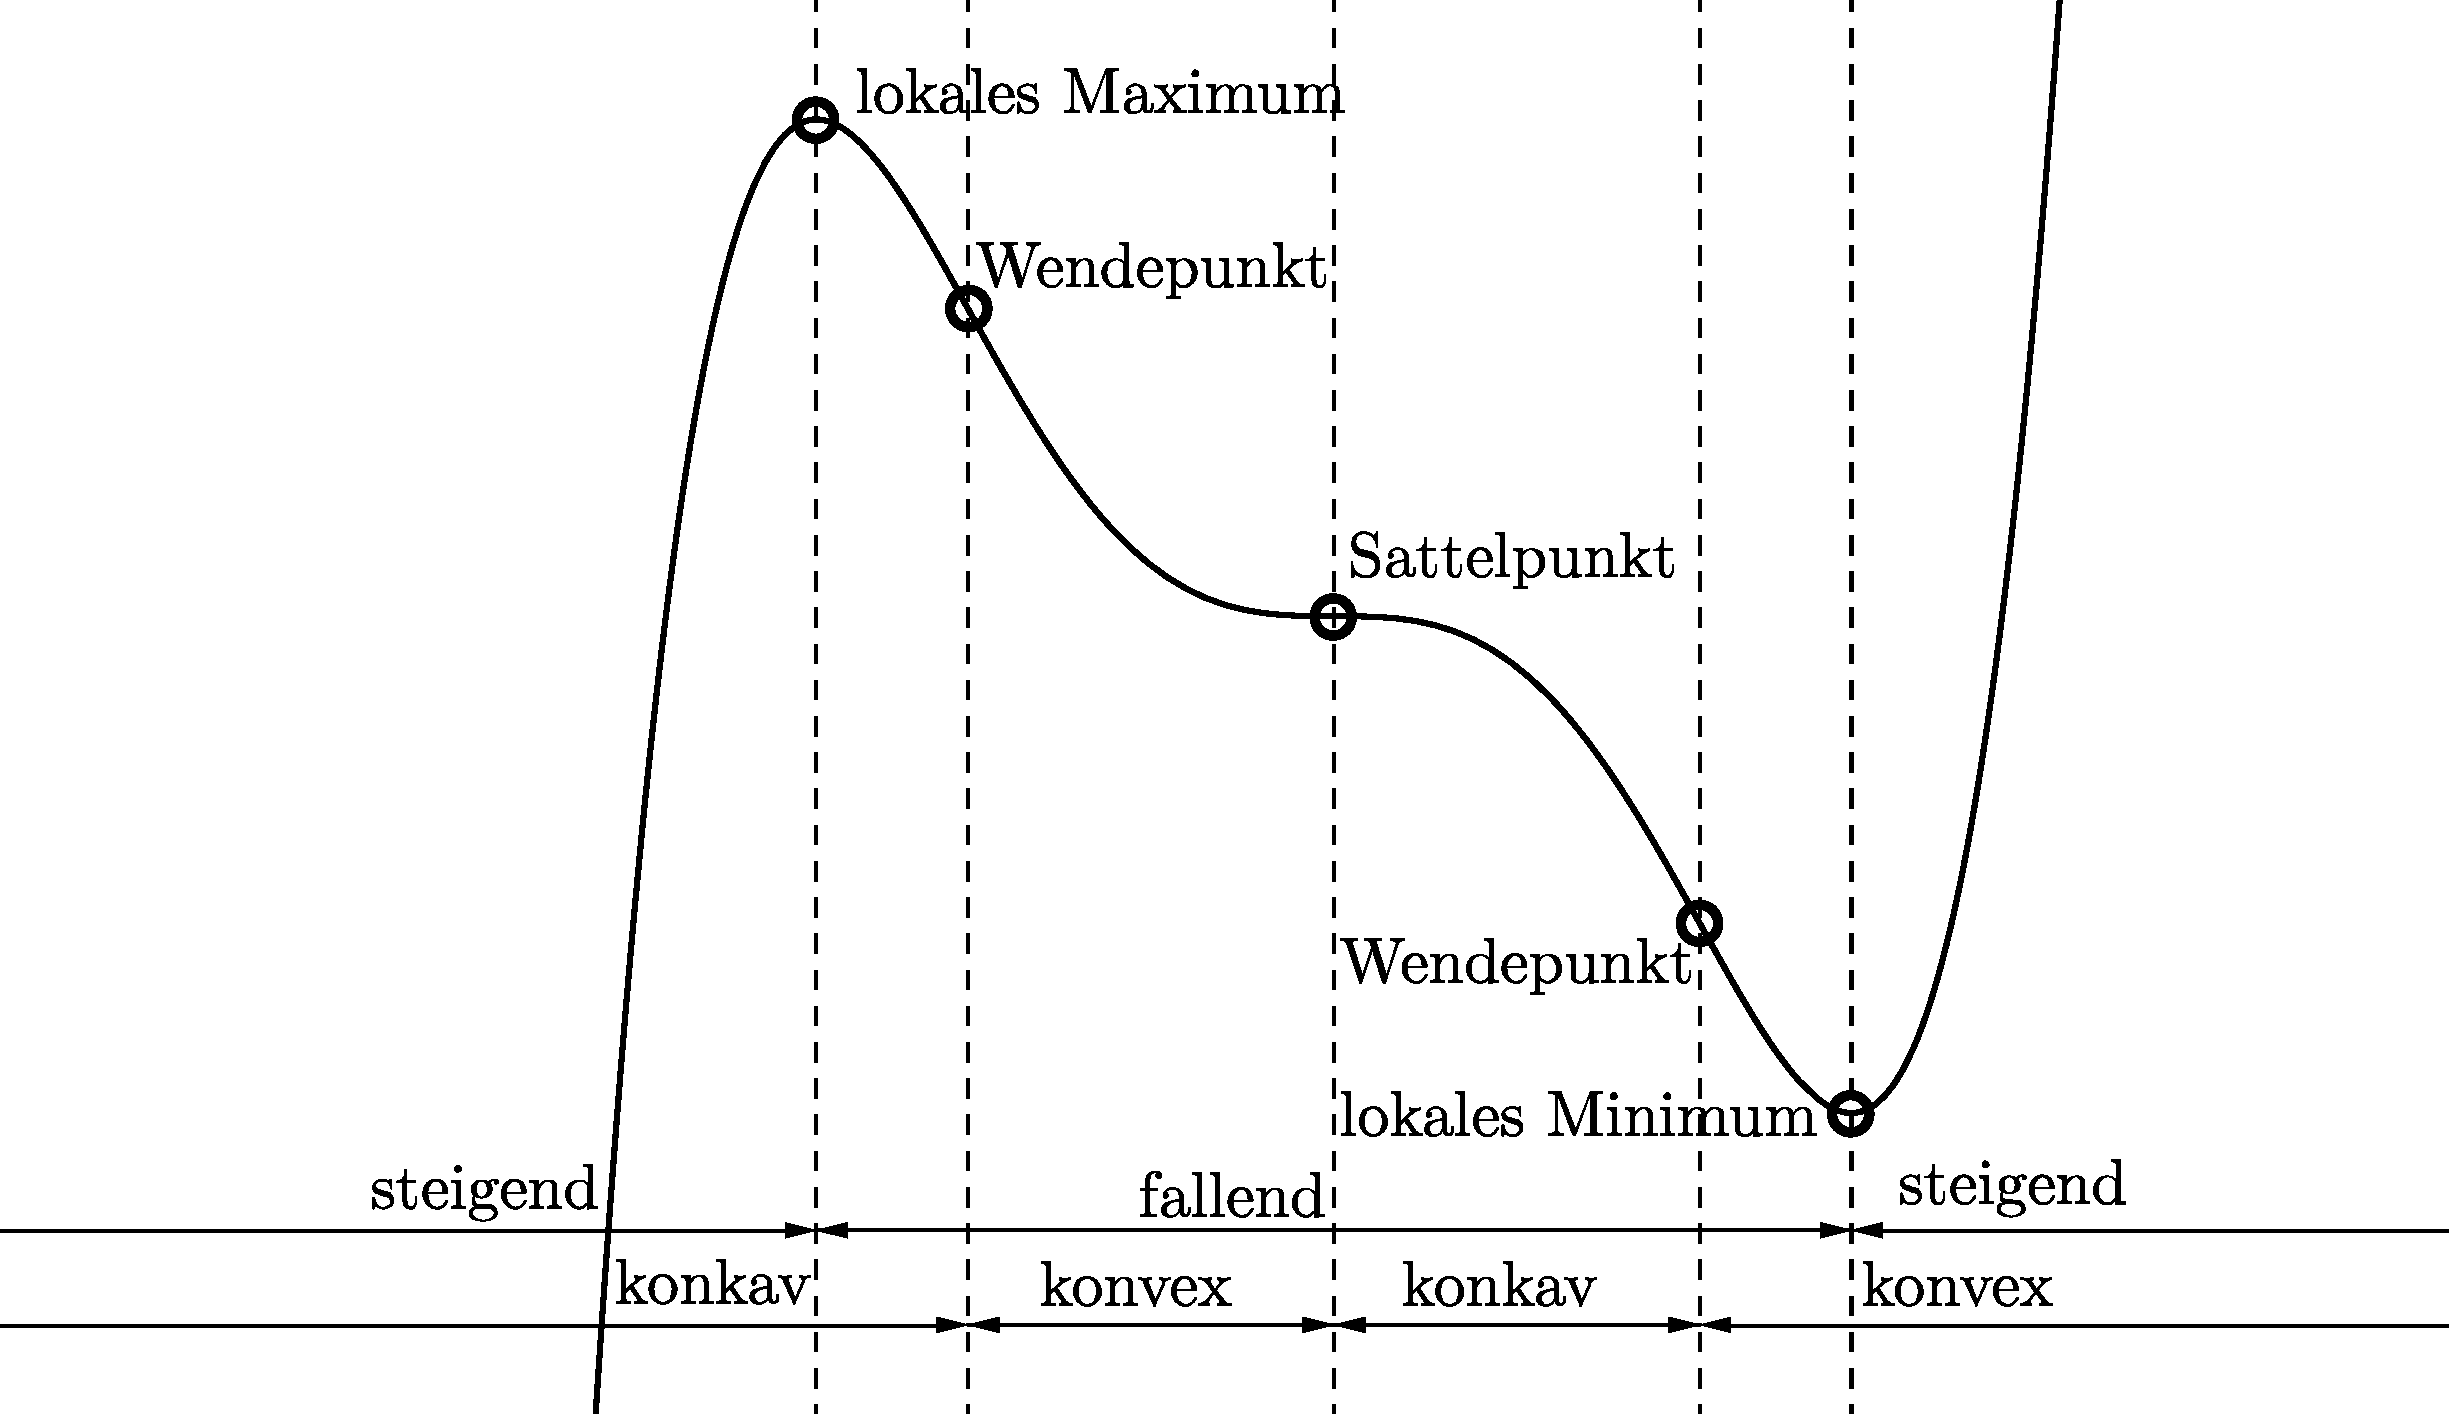
\includegraphics[width=0.88\textwidth]{kurvendiskussion.pdf}
\end{figure}
 
\end{document}

